\documentclass[shorttitlesize=55]{ees}

\shorttitle{Missa S. Wolfgangi}

\def\eesCommentaryAfterToe{\section{Acknowledgements}Permission of the Schottenstift Abbey Archive to use source \A1 for this edition is gratefully acknowledged. We thank Dr. Maximilian Alexander Trofaier for assistance in obtaining this source.}

\begin{document}

\eesTitlePage

\eesCriticalReport{
  – & –   & –    & Eybler likely revised \A1 at a later time,
                   which is evident from different ink colors
                   (initial version \A1a: lighter color;
                   revision \A1b: darker color).
                   Moreover, \B1 was copied from the initial version
                   (or a copy thereof).
                   Obvious mistakes in \B1 are not listed here. \\
  \midrule
  1 & –   & –    & tempo indication in \A1a: “Andante” \\
    & 58  & –    & \A1a ended with a \halfNoteDotted\ in ob and a
                   \quarterNote\ in the other parts.
                   In \A1b, Eybler shortened the 3rd \quarterNote\ to an
                   \eighthNote, added a fermata to the rest at the end of
                   the bar, and cancelled the subsequent full measure rest.
                   Notably, he did not correct the number of bars at
                   the end of the movement (which still reads “100”). \\
  \midrule
  2 & 117 & vl 2 & in \A1 \flat b′ instead of \sharp a′ \\
  \midrule
  3 & 50  & vl   & 11th \sixteenthNote\ in \A1: e″16 \\
    & 161–164 & – & In \A1, these bars have been heavily edited in the org
                   and vlne staff: The initial version (\B1, and thus likely
                   \A1a) was\newline
                   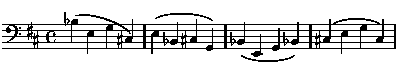
\includegraphics{snippet_1.pdf}\newline
                   The second version was\newline
                   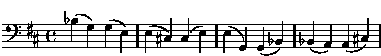
\includegraphics{snippet_2.pdf}\newline
                   The third version (entered in the T~staff) is reproduced
                   in this edition. Moreover, there is a fourth version,
                   where bars 161–164 have been cancelled with pencil.
                   However, the text “et mortuos” would be missing
                   in this version. \\
    & 177 & S    & grace note added by editor \\
  \midrule
  5 & 43–51 & –  & in \A1 indicated by vide marks and the directive
                   “Osanna da Capo dal Segno sin al Fine” \\
  \midrule
  6 & 64  & ob 2 & 2nd \quarterNote\ in \A1: a′4 \\
}

\eesToc{}

\eesScore

\end{document}
